\documentclass[border=10pt]{standalone}
\usepackage{tikz}
\usetikzlibrary{shapes, positioning}

\begin{document}
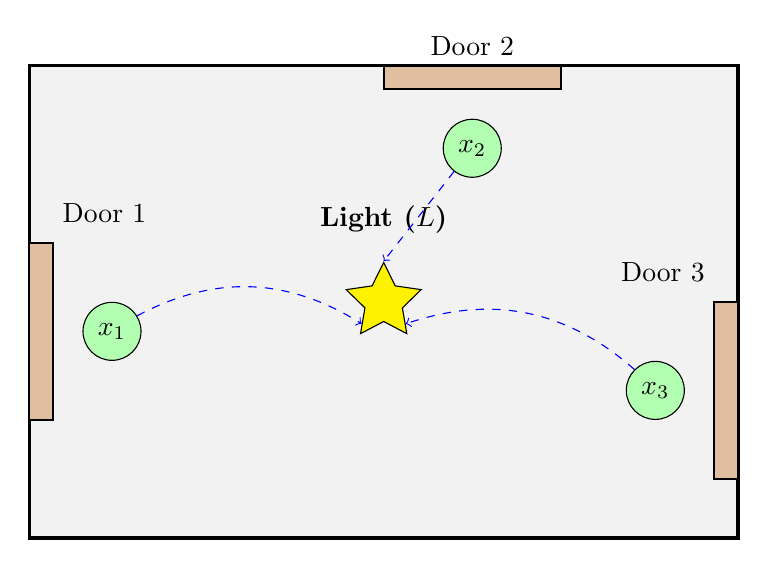
\begin{tikzpicture}[scale=1.5]

    % --- Room Outline ---
    \draw[very thick, fill=gray!10] (0, 0) rectangle (6, 4) node[midway] {};

    % --- Doors and Switches ---
    % Door 1 and Switch x1
    \draw[thick, fill=brown!50] (0, 1) rectangle (0.2, 2.5);
    \node[anchor=west] at (0.2, 2.75) {Door 1};
    \node[draw, circle, fill=green!30] (X1) at (0.7, 1.75) {$x_1$}; % Switch 1

    % Door 2 and Switch x2
    \draw[thick, fill=brown!50] (3, 4) rectangle (4.5, 3.8);
    \node[anchor=south] at (3.75, 4) {Door 2};
    \node[draw, circle, fill=green!30] (X2) at (3.75, 3.3) {$x_2$}; % Switch 2

    % Door 3 and Switch x3
    \draw[thick, fill=brown!50] (6, 0.5) rectangle (5.8, 2);
    \node[anchor=east] at (5.8, 2.25) {Door 3};
    \node[draw, circle, fill=green!30] (X3) at (5.3, 1.25) {$x_3$}; % Switch 3

    % --- Light Fixture (Output L) ---
    % The light is controlled by the logical XOR combination of all switches
    \node[star, star point ratio=2, inner sep=2pt, draw, fill=yellow, minimum size=1cm] (L) at (3, 2) {};
    \node[anchor=south] at (3, 2.5) {\textbf{Light ($L$)}};

    % --- Wiring Concept (Logic Connection) ---
    % Indicate that the switches are logically connected to the light's control mechanism
    \draw[->, dashed, blue] (X1) to[bend left] (L.south west);
    \draw[->, dashed, blue] (X2) to (L.north);
    \draw[->, dashed, blue] (X3) to[bend right] (L.south east);
    


\end{tikzpicture}
\end{document}